% ============================================================
\section{Results}
% ============================================================

Every figure below comes from 100 seeds per cell at $T=20\,000$ steps, with percentile bootstrap intervals. Raw continuity values are
primary; \eqref{eq:delta} and \eqref{eq:rho} are derived from them, with
intervals propagated by bootstrapping each arm separately.

\subsection{The substrate behaves like an evolving population}

All five validation checks pass (Figure~\ref{fig:valid}). Across 6 combinations of $k_c$ and $R$ the measured
equilibrium affinity matches the interior optimum of \eqref{eq:ess} to
within 0.3\%, and $R/S$ under imposed truncation
selection departs from the breeder's prediction of unity by at most
$0.001$.

Drift is present and its timescale grows with population size,
but the scaling is sublinear and we cannot say why. Reproductive
variance does not account for it: $V_k$ is approximately
constant at 1.89, so $N_e\approx4N/(V_k+2)$
predicts $N_e\approx N$ while the measured value is 0.30--0.52 of it, and
nor does \citet{hill1972}'s correction for overlapping
generations, which would bite only if the generation interval
grew with $N$ and it does not (0.22--0.38). Two independent estimates of $N_e$, from
the decay of marker variance and from its equilibrium value
under mutation, agree at matched census size and horizon within
a factor of 1.2--2.2, so
the fourth check is no longer tautological even though the
deficit stands unexplained. Cohort and generation-interval
measurements, including the falsification of the
overlapping-generation correction, are in the supplementary
material.

The structural identities hold in all 10 grid variants in which the manipulated rule fires; in 1 further variant it is degenerate rather than
broken, the reproductive threshold sitting below the contribution one so
that almost nobody becomes a donor. We require the identities and report
the effect size without requiring it, since demanding that withdrawal
always bite would demand that an extrinsic rule always matter.

\begin{figure}[ht]
\centering
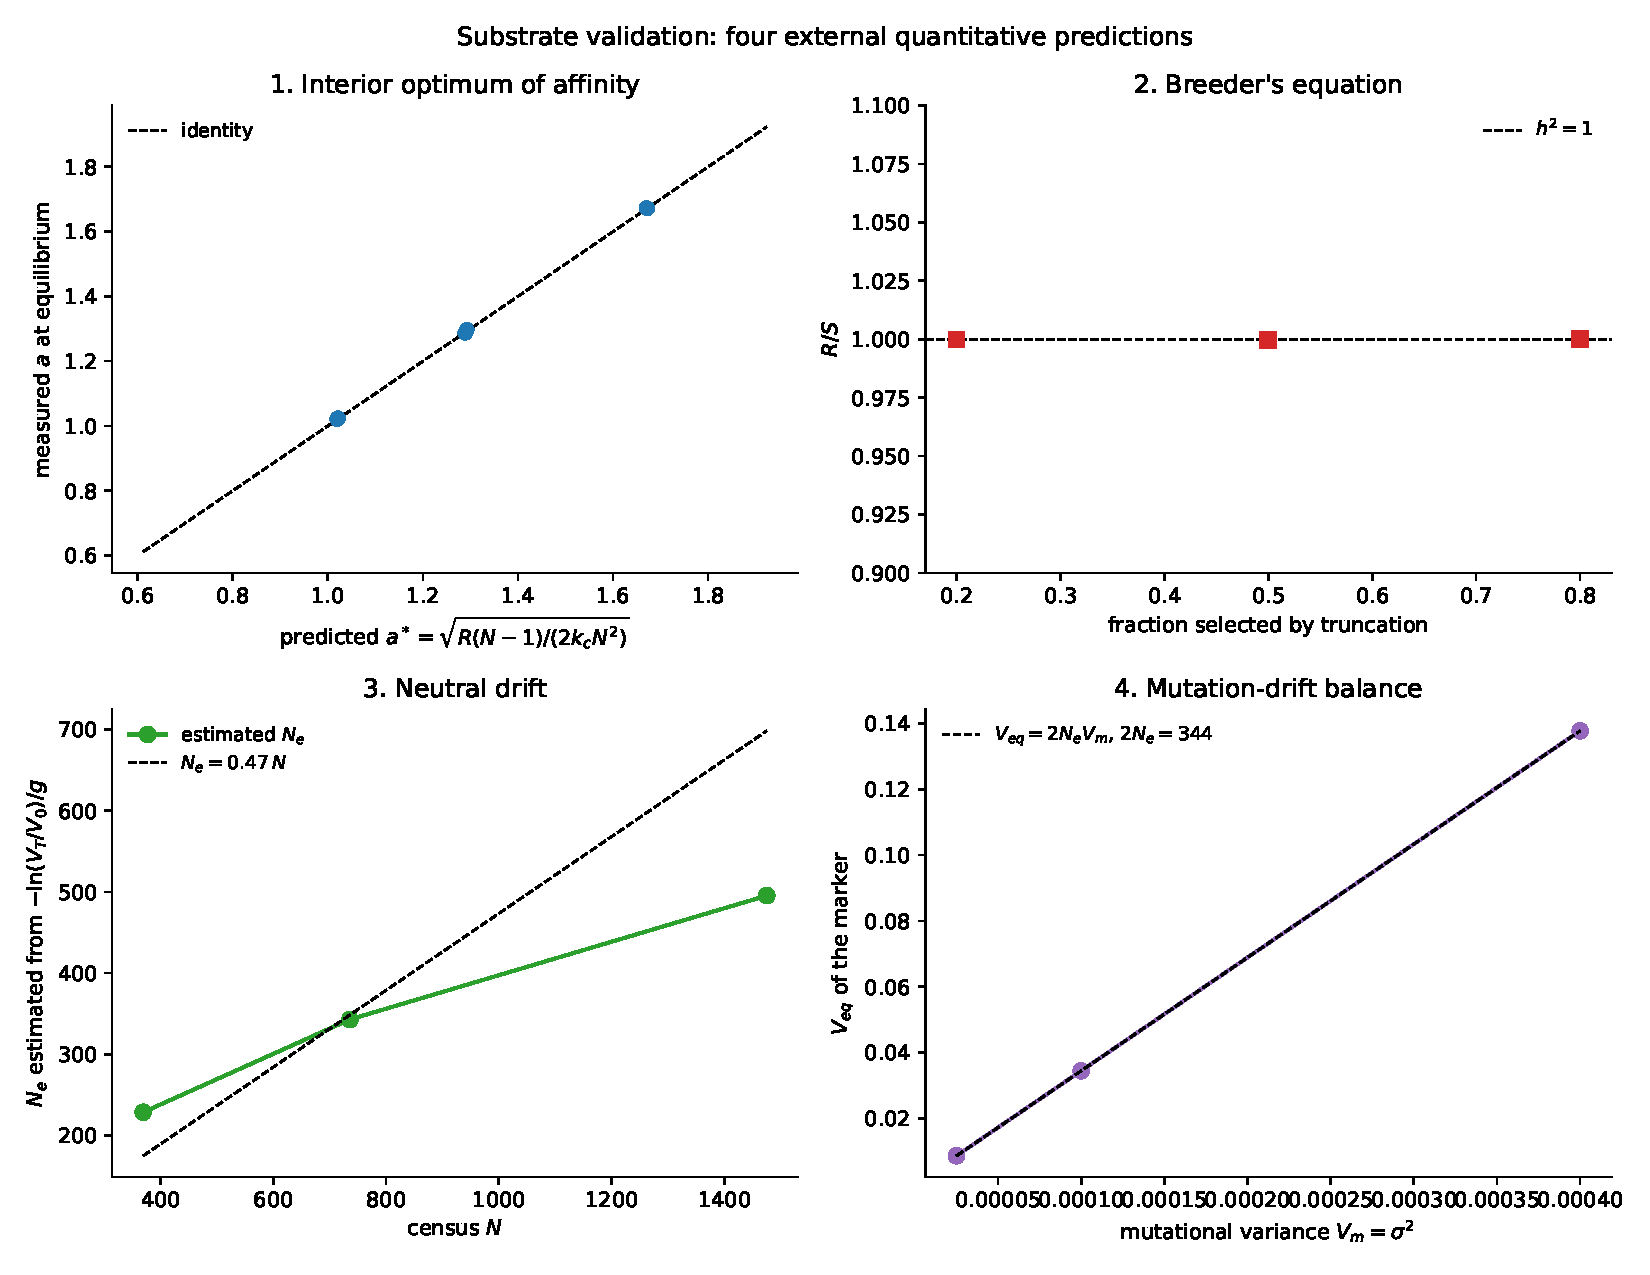
\includegraphics[width=0.94\linewidth]{fig_validacion}
\caption{Substrate validation against four external quantitative predictions: the analytic evolutionarily stable affinity, the breeder's equation, the relationship between effective and census population size, and the scaling of equilibrium marker variance with mutational variance.}
\label{fig:valid}
\end{figure}

\subsection{Neither coordinate has a dynamical signature at baseline}

In monoculture the four conditions are \textbf{bit-for-bit identical}:
same births, same deaths, same final population, same mean genome, in
100 of 100 seeds. This is a
determinism check rather than a statistical one---a seed either yields
four identical trajectories or it does not, and a single discrepancy
would falsify the claim---so it needs no interval and admits no
dispersion.

The reason is the one \eqref{eq:neq} exists to name. A rule conditioned on
the label has nobody to disfavour when everyone carries the same label, so
it reduces to its unconditioned form. And an extrinsic rule applying the
same criterion at the same moment as its intrinsic counterpart produces
the same allocations. \emph{The coordinates are properties of rules, not
of trajectories.} They are invisible until the intervention that
interrogates them is run---which is the substantive reason an audit
(\S4) cannot be replaced by watching a system behave.

\subsection{Each intervention responds to exactly one coordinate}

\begin{table}[ht]
\centering\small
\caption{The two interventions are orthogonal to each other. Withdrawing
the external operator moves only the control coordinate; relabelling the
recipient moves only the exchangeability coordinate. Point estimates with
95\% bootstrap intervals.}
\label{tab:orto}
\begin{tabular}{lccrr}
\toprule
\textbf{Condition} & $C$ & $A$ & \textbf{Operator removal} $\Phi_R/\Phi_B$ & \textbf{Relabelling} $L_1/L_0$\\
\midrule
$\mathrm{I/x}$ & I & 0 & 1.000~[0.993,\,1.007] & 0.989~[0.974,\,1.004]\\
$\mathrm{I/p}$ & I & 1 & 1.000~[0.993,\,1.007] & 0.000~[0.000,\,0.000]\\
$\mathrm{E/x}$ & E & 0 & 1.143~[1.134,\,1.152] & 0.989~[0.974,\,1.004]\\
$\mathrm{E/p}$ & E & 1 & 1.143~[1.134,\,1.152] & 0.000~[0.000,\,0.000]\\
\bottomrule
\end{tabular}
\end{table}

\begin{figure}[ht]
\centering
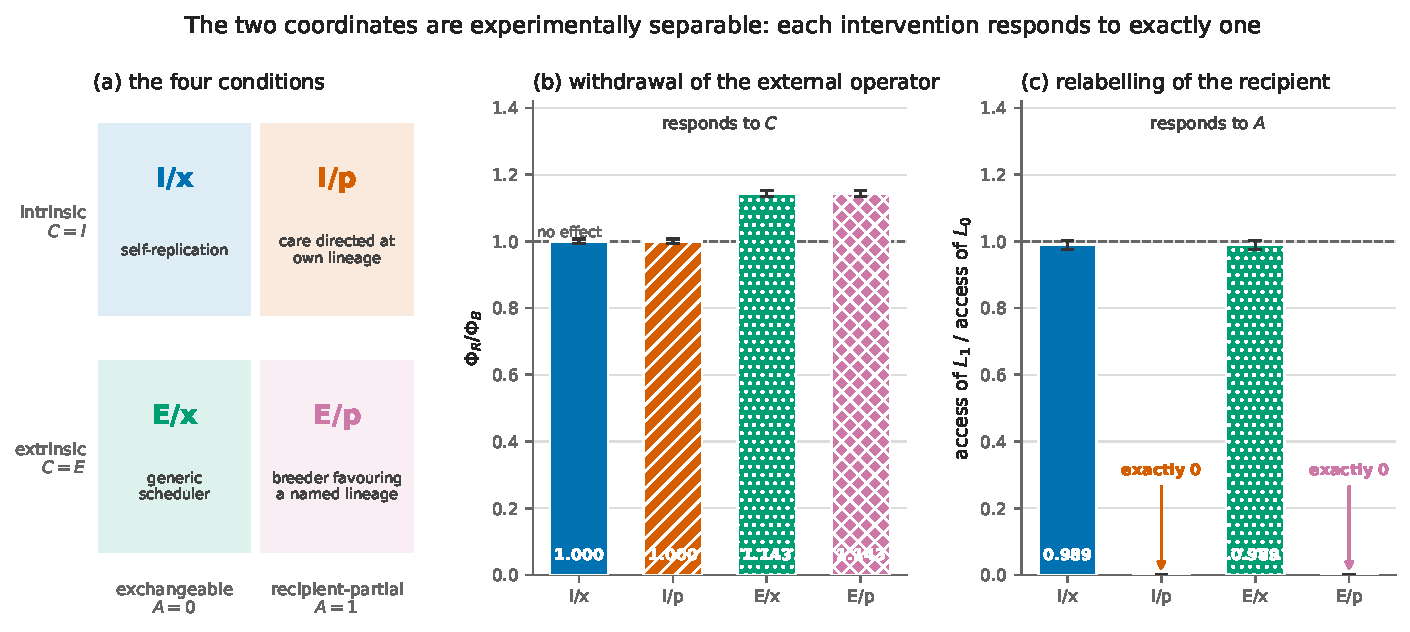
\includegraphics[width=1.0\linewidth]{fig1_ortogonalidad}
\caption{The two coordinates are experimentally separable. (a) The four conditions differ from their neighbours in exactly one thing. (b) Withdrawing the externally operated supply leaves the intrinsic conditions at exactly $1.000$ and moves both extrinsic ones. (c) Relabelling the recipient leaves the exchangeable conditions unchanged and drives allocation to the relabelled lineage to exactly zero in both partial ones. Bars carry 95\% bootstrap intervals; hatching encodes condition so identity never rests on colour alone.}
\label{fig:orto}
\end{figure}

Table~\ref{tab:orto} and Figure~\ref{fig:orto} are the experimental
content of \eqref{eq:twoaxes}. They are construct validation: the four
rules were built to differ in one thing each, so a clean separation is
partly a property of the design. What it establishes is that the
coordinates \emph{can} be manipulated independently, which was in doubt.
Withdrawing the externally operated supply leaves the two intrinsic
conditions at a ratio of exactly $1.000$ with zero dispersion across
seeds---there is no external machinery to withdraw---while both extrinsic
conditions move. Relabelling leaves the two exchangeable conditions
unchanged and drives allocation to the relabelled lineage to exactly zero
in both partial ones.

The zeros are worth dwelling on. They are not small numbers with
intervals that happen to include zero; they are exact, because the rule's
domain excludes the label and no sampling variation can put it back. A
binary $A$ is the honest report of a binary fact.

\subsection{Two things the framework got wrong}

Running the framework rather than only arguing it turned up two defects
in it. Both are reported here, in one place, because they are findings
of the experiment rather than caveats on it: the first concerns what the
exchangeability coordinate fails to distinguish, and the second, in
\S6.5, concerns the range of the normalized substitution contrast.
Neither is patched.

\paragraph{Exclusion and partition share a coordinate and have opposite
outcomes}
The two partial cells share a coordinate and behave in opposite ways, and
the framework as stated does not distinguish them.
Figure~\ref{fig:relabel} shows both panels of it.
Under $\mathrm{E/p}$ a single allocator conditioned on identity excludes:
the relabelled lineage receives nothing from anyone. Under
$\mathrm{I/p}$ each donor serves its own label, so the relabelled lineage
receives---but only from itself. Allocation across the label boundary is
exactly zero in both; aggregate supply to the relabelled lineage is zero
in one and positive in the other.

This is a genuine gap in the account of \S2, found by running it. The
coordinate $A$ answers whether a rule's allocation depends on recipient
identity. It does not answer whether the resulting partition leaves the
disfavoured lineage with a viable supply of its own, and those come apart
in the most ordinary case in biology: identity-keyed care partitions a
population without starving anybody's offspring but their own kin's
competitors. A graded $A$ may capture part of this distinction but is
not guaranteed to resolve it: the difference may be one of the topology
of the allocation rather than of the intensity of partiality.

\begin{figure}[ht]
\centering
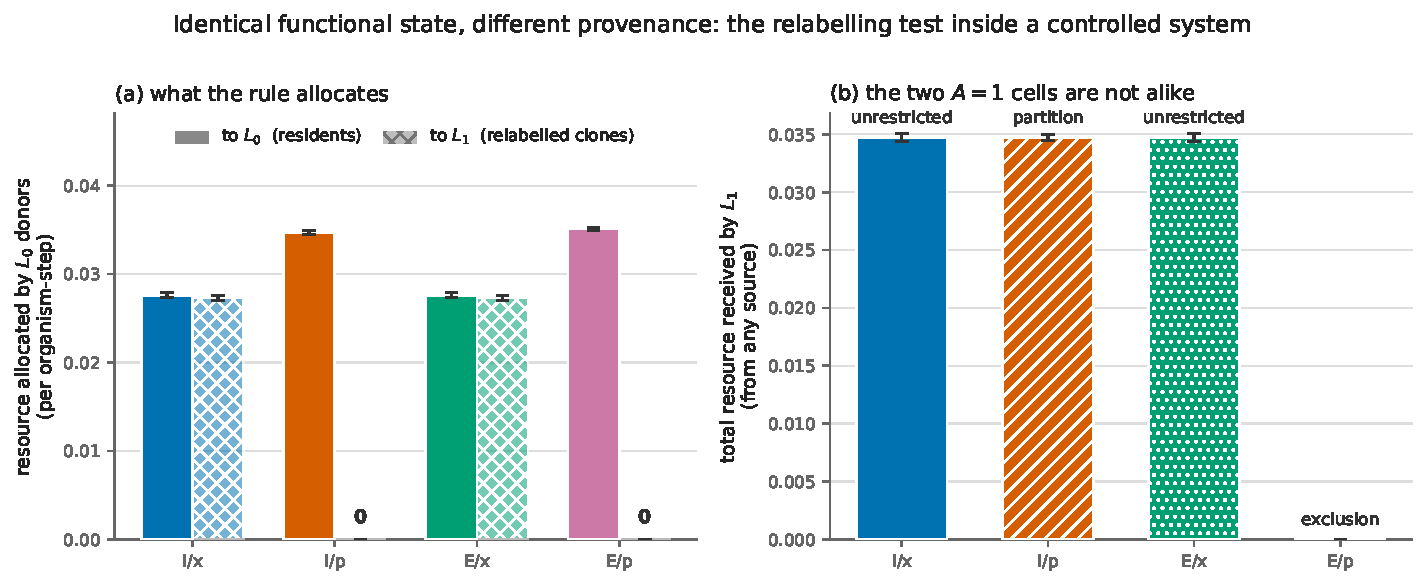
\includegraphics[width=0.92\linewidth]{fig2_reetiquetado}
\caption{Identical functional state, different provenance. (a) What the rule allocates to residents and to relabelled clones, per organism-step, in a short window after injection. (b) Total supply reaching the relabelled lineage from any source: the two $A=1$ cells share a coordinate and differ completely, one excluding and the other partitioning.}
\label{fig:relabel}
\end{figure}

\subsection{The range of \texorpdfstring{$\rho$}{rho}, what the data do not separate, and a principled \texttt{NA}}

\begin{table}[ht]
\centering\small
\caption{The three arms, at the largest competing-lineage size tested ($n_{L_1}=200$ of 400). $\Phi$ is autonomous reproductive cycles completed by the focal
lineage, with 95\% bootstrap intervals. Arm S is matched to arm B on
emitted volume for the resource manipulation; for the suppression
manipulation no defensible match exists and the entry is the range of
$\rho$ over the substitute's whole intensity range, for the reasons
given under matching. The acquisition cost paid in arm S is reported
separately and never absorbed into $\Phi$.}
\label{tab:brazos}
\begin{tabular}{lrrrcc}
\toprule
\textbf{Manipulation} & $\Phi_B$ & $\Phi_R$ & $\Phi_S$ & $\delta$ & $\rho$\\
\midrule
Partial transfer (negative control) & 149\,192 & 77\,389 & 78\,848 & +0.48 & 0.98~[0.82,\,1.19]\\
Reproductive resource & 168\,214 & 78\,848 & 80\,979 & +0.53 & 0.98~[0.86,\,1.11]\\
Competitor suppression & 151\,506 & 78\,848 & 85\,309 & +0.48 & 0.91--1.10\\
\bottomrule
\end{tabular}
\end{table}

Throughout this section $\rho$ is the normalized substitution contrast
of \eqref{eq:rho}, not a fraction: zero and one are reference points
and values above one are meaningful.

Table~\ref{tab:brazos} reports the three manipulations at the largest
competing-lineage size and Figure~\ref{fig:brazos} the raw continuity
values behind them; the dose-response below gives the rest. One
bookkeeping point, so that nothing is counted twice: the baseline and
removal arms of the first manipulation at $n_{L_1}=0$ are the same
measurement as the $\mathrm{E}$ rows of Table~\ref{tab:orto}, not an
independent replication of it.

\paragraph{The negative control, and a pre-registered prediction that
failed} We pre-registered that the partial transfer rule would return
$\rho=\texttt{NA}$ throughout, because the audit calls it
recipient-partial while baseline dependence on it is not positive. It
does so at $n_{L_1}\in\{0, 40\}$: at
$n_{L_1}=0$ the supply is a \emph{constraint} rather than a support
($\delta=-0.125$, withdrawing it raises
the autonomous cycle count---a property of the transfer being
externally operated rather than of its partiality, as \S6.6 sets out),
so there is no demonstrated dependence to
apportion and the honest output is not a number. That is \eqref{eq:neq}
measured rather than argued: $A=1$ with $\rho=\texttt{NA}$ is a real
state of affairs, and a method reporting $\rho=0$ there would turn the
absence of demonstrated dependence into a spurious estimate of
complete restoration.

At $n_{L_1}\in\{100, 200\}$ the
prediction fails, and the reason is worth more than the prediction
was. A partial allocation rule in a mixed population is not only a
support that might turn out to be unnecessary; it is also a
\emph{competitor-suppression mechanism}, because the non-focal
lineage contributes to the pool and is not served. Once the
competitor is large enough, withdrawing the rule releases it and
harms the focal lineage, so baseline dependence becomes positive.
The negative control and the suppression manipulation converge at
high dose---which is a finding about what partial allocation
\emph{is}, not a defect of either.

\paragraph{\texorpdfstring{$\rho$}{rho} above one: the second defect}
At $n_{L_1}=100$ the negative control returns
$\rho=1.66~[1.07,\,3.04]$, whose interval excludes one from
below---which the normalized substitution contrast permits, since
it is not a fraction and has no upper bound. $\rho>1$ means
$\Phi_S<\Phi_R$: de-personalising the rule costs the focal lineage more
than withdrawing it altogether, because the open substitute does not
merely stop favouring the focal lineage---it supplies the rivals the
partial rule was excluding. \S3.5 now states the unbounded range and
what values above one mean.

\paragraph{The range of \texorpdfstring{$\rho$}{rho}, and what the data do not separate}
The range is established within the resource manipulation, along the
dose, not by contrasting manipulations. At $n_{L_1}=0$
$\rho=-0.02~[-0.10,\,0.05]$ and at $n_{L_1}=200$
$\rho=0.98~[0.86,\,1.11]$; the two intervals are disjoint.
So the contrast moves from about its zero reference point to about its
one, driven by a quantity we control.

What the data do \emph{not} support is a separation between the
manipulations at the largest dose. There all three intervals cover one and every pair overlaps, so at
$n_{L_1}=200$ we cannot distinguish a rule whose benefit
was the resource from one whose benefit was the exemption. An
earlier run at thirty seeds appeared to separate them; it did not
survive the increase to 100. We report the
convergence rather than the appearance.

The convergence has a mechanism rather than being an artefact of the
estimator: as the competing lineage grows, what the partial provider
withholds from it becomes a larger part of what the focal lineage
enjoys, so supplying a resource and suppressing a competitor converge
on being the same intervention.

\paragraph{The dose-response, and where \texorpdfstring{\texttt{NA}}{NA} comes back}
Varying the size of the competing lineage moves $\rho$ systematically:
\begin{center}\small
\begin{tabular}{rccc}
\toprule
$n_{L_1}$ & Partial transfer & Reproductive resource & Competitor suppression\\
\midrule
0 & \texttt{NA} & -0.02 & \texttt{NA}\\
40 & \texttt{NA} & 0.50 & 0.92--1.73\\
100 & 1.66 & 0.85 & 0.91--1.27\\
200 & 0.98 & 0.98 & 0.91--1.10\\
\bottomrule
\end{tabular}
\end{center}

At $n_{L_1}=0$ the partial rule has nobody to disfavour and $\rho$ is
undefined in the two manipulations whose baseline dependence vanishes
there. That is the limiting case of the monoculture identity of \S6.2,
and it is the clearest statement the experiment produces:
\emph{partiality needs someone to disfavour before it can matter to
anything}.

The resource curve rises monotonically and approaches one from below rather than
plateauing short of it; an apparent plateau at thirty seeds did not
survive. The approach to one is expected here, since $\rho=1$ is the
point at which none of this manipulation's dependence survives
de-personalising the rule.

\paragraph{A support that was a constraint}
\S3.5 predicts that $\delta$ can be negative, and it is: at
$n_{L_1}=0$ the externally operated transfer
gives $\delta=-0.125~[-0.132,\,-0.118]$, strictly below zero,
and withdrawing it leaves the lineage completing about 14\% \emph{more} reproductive cycles. Table~\ref{tab:orto} gives the
identical ratio for $\mathrm{E/x}$ and $\mathrm{E/p}$, so the
constraint belongs to the transfer being \emph{operated from
outside} rather than to its partiality, and applies to both
extrinsic cells. The mechanism agrees: levelling reserves costs the
individuals closest to reproducing more than it gains those
furthest from it, which is about the allocation, not the label. A
framework reading every external supply as support would have
scored this one backwards; the sign of $\delta$ is what stops it.

\begin{figure}[ht]
\centering
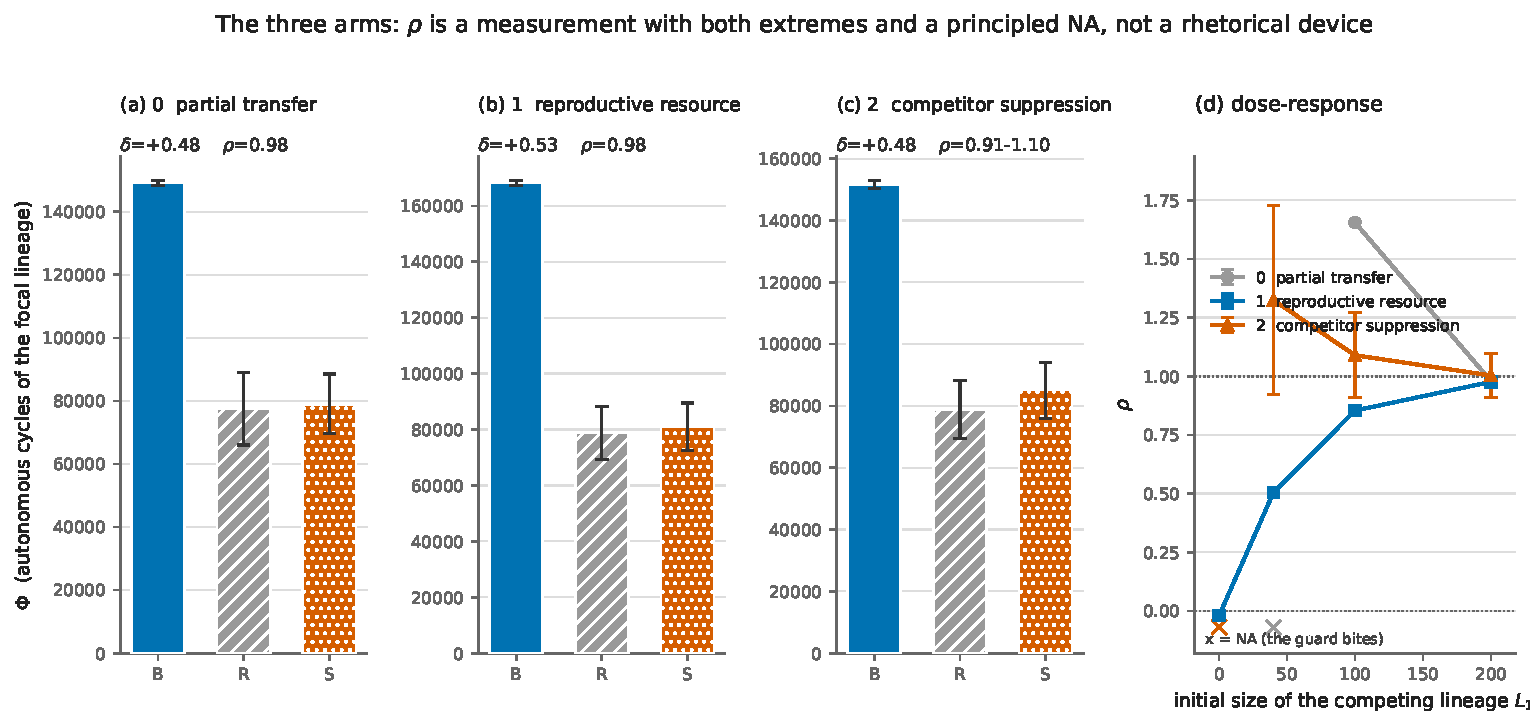
\includegraphics[width=1.0\linewidth]{fig3_brazos}
\caption{The three arms. (a)--(c) Raw continuity in each arm, which is the primary result; $\delta$ and $\rho$ are derived from it. (d) $\rho$ against the size of the competing lineage, with crosses marking the doses at which the guard bites and the honest output is \texttt{NA} rather than zero.}
\label{fig:brazos}
\end{figure}

\paragraph{Matching, and where we could not achieve it}
Calibration used pilot seeds disjoint from the confirmatory ones and was
discarded. For the provider the matched quantity is directly
controllable: at $n_{L_1}=200$ the substitute emitted 680\,083 units against a target of 680\,083 (0.0\% error). The acquisition cost recipients paid to qualify was 0.12 times the volume received; that is the price of an open rule and it
belongs in the report, not in $\Phi$.

For the suppression manipulation we could not construct a defensible
match, and say so rather than presenting one. The obvious target---the
fraction of reproduction the rule prevents---turned out to be unusable
twice over. A counter of blocked events counts organism-steps rather
than prevented events, and the partial rule sterilises a sublineage
permanently, so its blocked individuals accumulate in a way the open
rule's do not; the two arms inflate by different factors. Retargeting to
realised reproduction, which counts events once, the calibration
converges to within $0.2\%$---but onto a quantity that is nearly
\emph{insensitive} to the manipulation, because the world compensates:
total births move by under $3\%$ while the substitute's intensity
ranges over two orders of magnitude. Fractions that differ by $100\times$
match equally well, and choosing between them would be arbitrary.

Matching on an insensitive quantity is not matching. We therefore report
$\rho$ across the substitute's whole range instead of at one calibrated
point. It stays near one throughout, so the conclusion is robust to a
matching choice we do not know how to make uniquely. That is a weaker
claim than the pre-registered one and a more defensible one, and it is
recorded as a deviation in the pre-registration.

\subsection{Does the open rule play favourites in effect?}

An exchangeable rule can still serve a systematically
better-endowed subset. Under \eqref{eq:exch} that is not
partiality---the rule is symmetric under relabelling and its
behaviour tracks state---but it is the exact edge of the
criterion, so we measured it. Observing who is served at each
moment, the open rule's recipients hold 47\% more reserve than the unserved, show no detectable difference in
affinity (0.1\% less), and sit at the 0.50 energy percentile---the median, not
the top. The excluded are the 1.3\% below the qualifying threshold, overwhelmingly newborns, and
the exclusion is transient.
Under the partial rule the recipients instead hold 6.8\% less reserve than the unserved, selected on
a label no amount of reserve can change.
So the answer is no: the open rule gates on a state anyone
reaches rather than concentrating on the fittest, and the
distinction \S2.2 draws between state-dependence and
identity-dependence survives contact with the data.

\subsection{The audited systems as profiles}

Figure~\ref{fig:perfil} shows the audit of \S4 as one coordinate per
function per system, with no aggregation. Two things are legible in it
that a summary index would hide. The canonical genetic algorithm and
the population-evolved language models are identical cell by cell,
three decades apart: the coincidence is seen rather than asserted. And
incomparability is read by comparing rows---among the rows audited
here, no artificial one
dominates the replicator's and the sovereign agents' both, whichever
value the indeterminate entry takes, while the free-living population
dominates each of them, which is the comparison the biological rows are
there to provide. These eight systems are spread across the space of
profiles rather than ordered along one; whether evolutionary systems at
large are so spread is not something eight cases can settle.

\begin{figure}[ht]
\centering
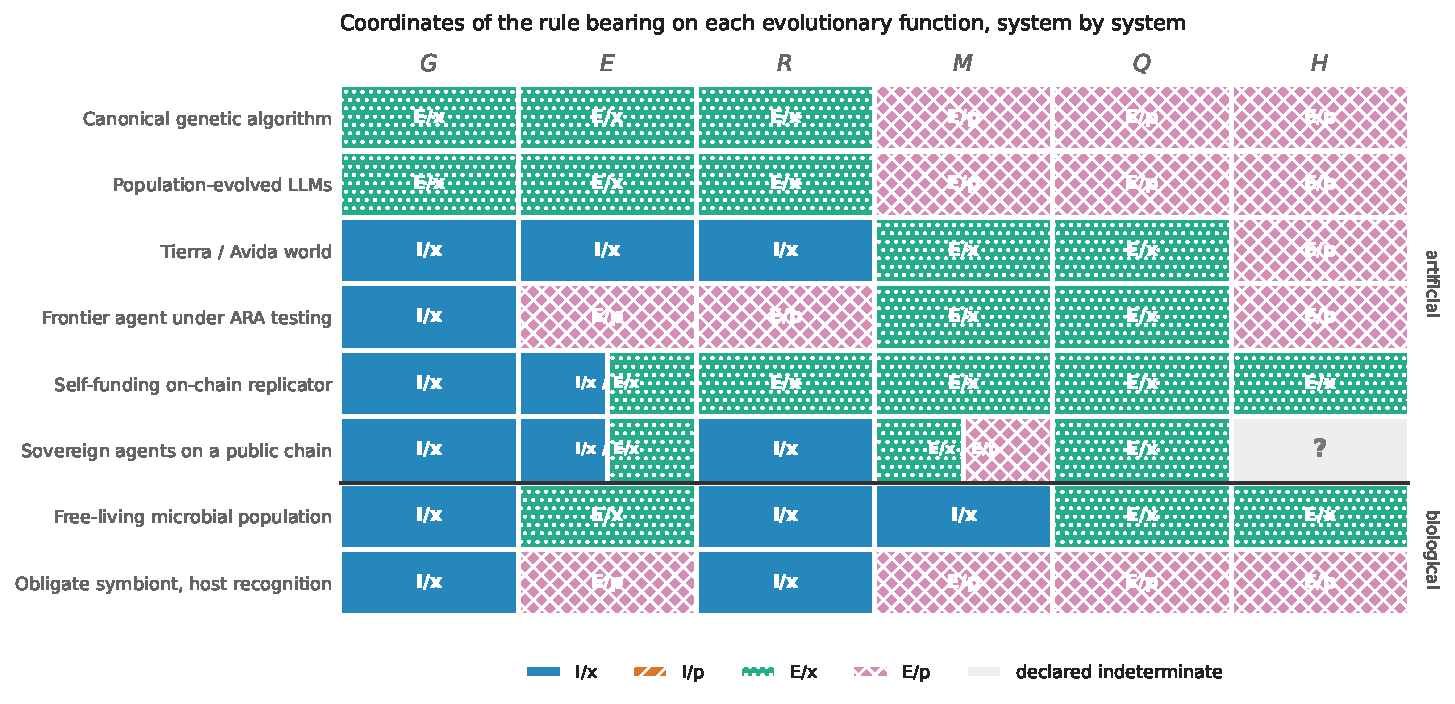
\includegraphics[width=1.0\linewidth]{fig4_perfil}
\caption{Each cell is the coordinate pair of the rule bearing on that function, transcribed from Table~\ref{tab:audit} and from nothing else. Split cells are functions served by two rules with different coordinates; the grey cell is the habitat entry declared indeterminate there. There are no numeric axes and no aggregation: \S2.5 gives no principled weights, so none are used.}
\label{fig:perfil}
\end{figure}

